% Created 2021-04-04 dim. 02:13
% Intended LaTeX compiler: pdflatex
\documentclass[a4paper,12pt]{article}
\usepackage[position=top,labelformat=empty]{subfig}
\usepackage{caption}
\usepackage[hmargin=2cm,vmargin=3cm]{geometry}


\usepackage{amsmath}
\usepackage{caption,graphicx,subcaption}
\usepackage[boxed]{algorithm2e}
\usepackage{authblk,tikz}
\usetikzlibrary{arrows,positioning}
\tikzset{
>=stealth',
pil/.style={ ->, thick, shorten <=2pt, shorten >=2pt,}}
\author[]{Vaitea Opuu}
\author[]{Nono S. C. Merleau}
\author[]{Matteo Smerlak}
\affil[]{Max Planck Institute for Mathematics in the Sciences, Leipzig, Germany}
\date{\today}
\title{Supplementary material: RNA fast-folding paths}
\begin{document}

\maketitle
\begin{figure}[!ht]
  \centering
  \subfloat[]{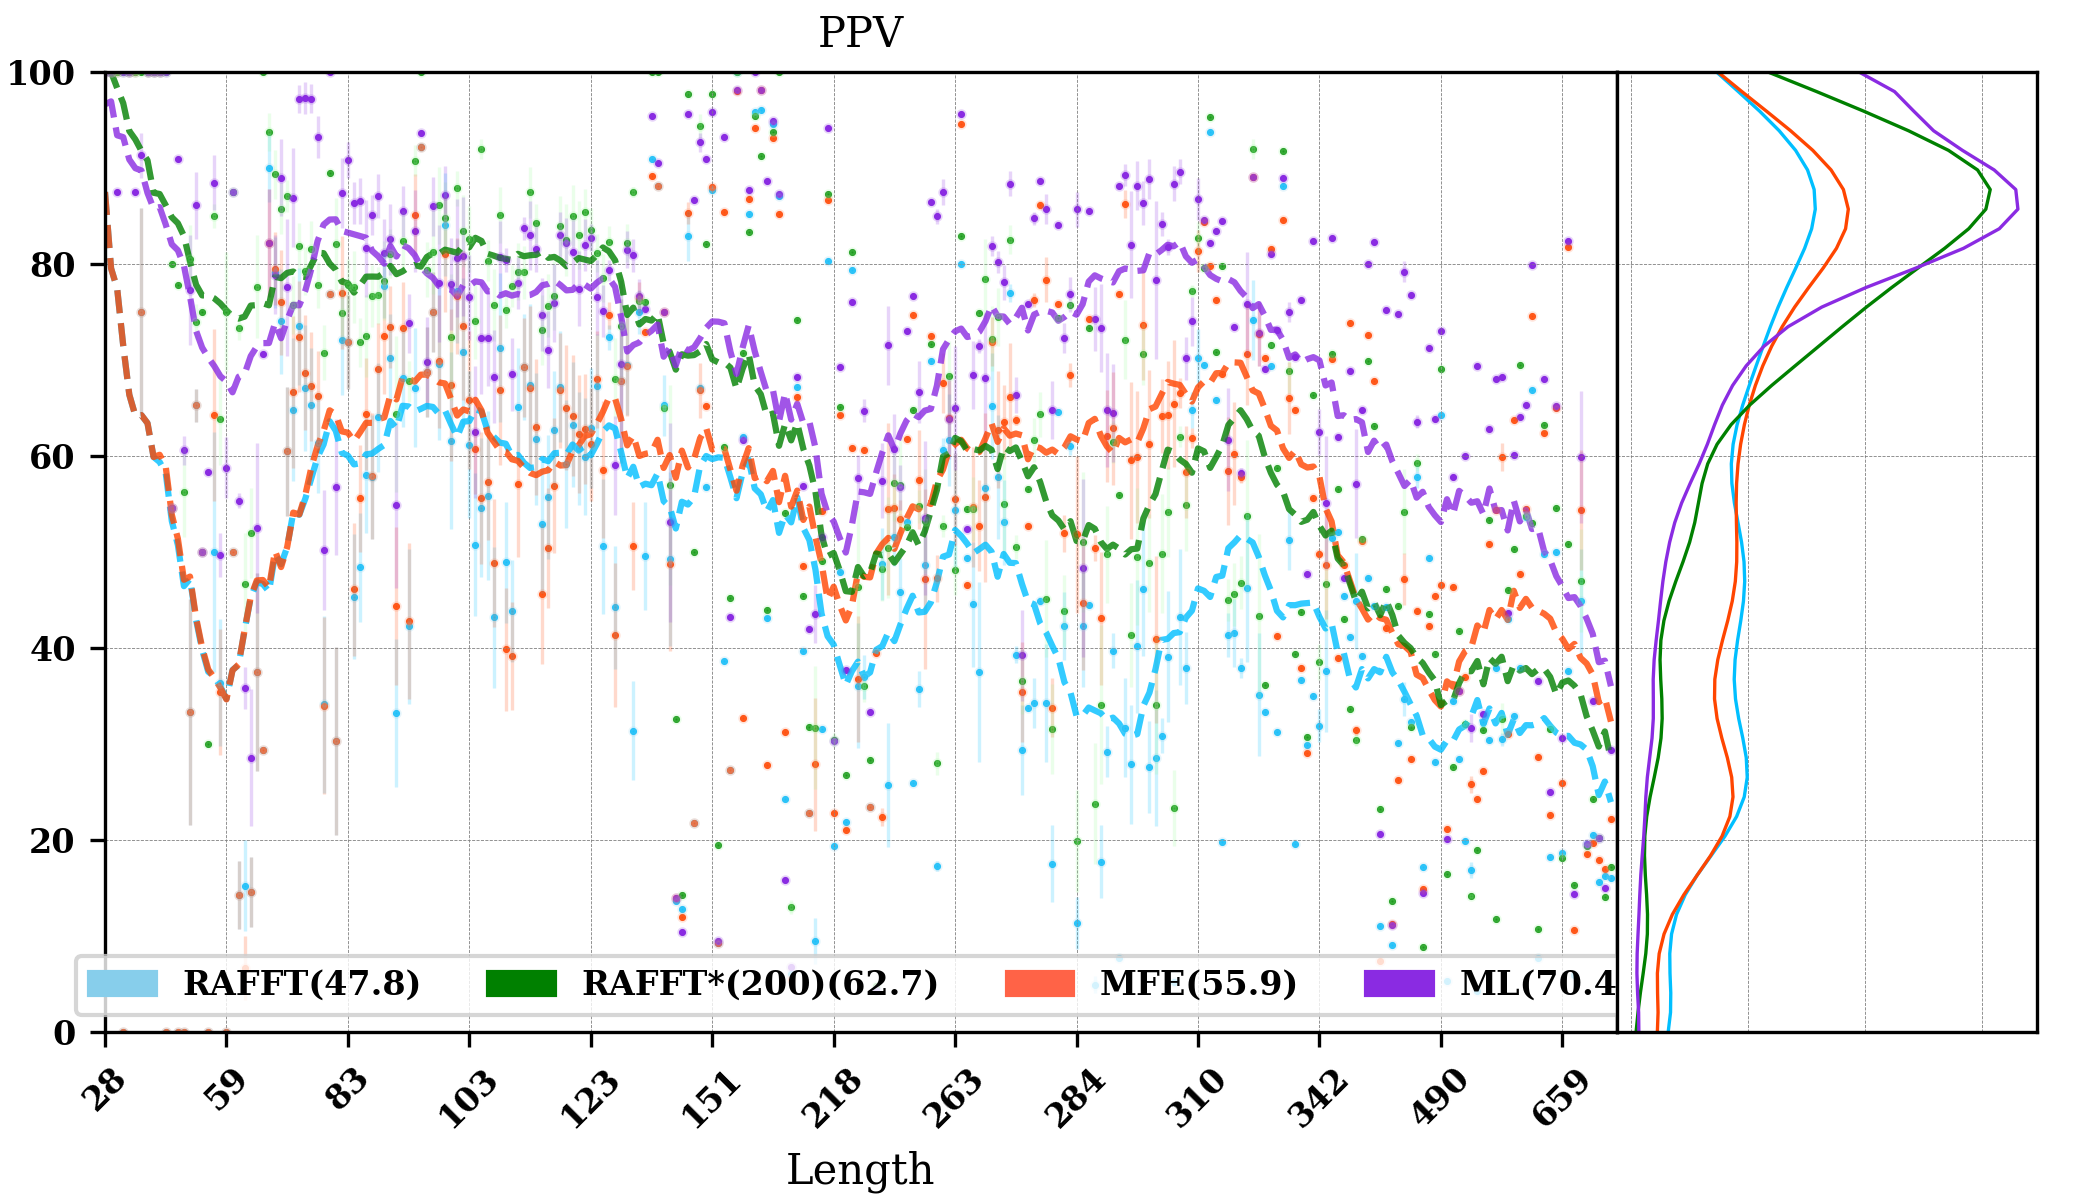
\includegraphics[scale=0.5]{img/fold_perf_ppv_200.png}}\\
  \subfloat[]{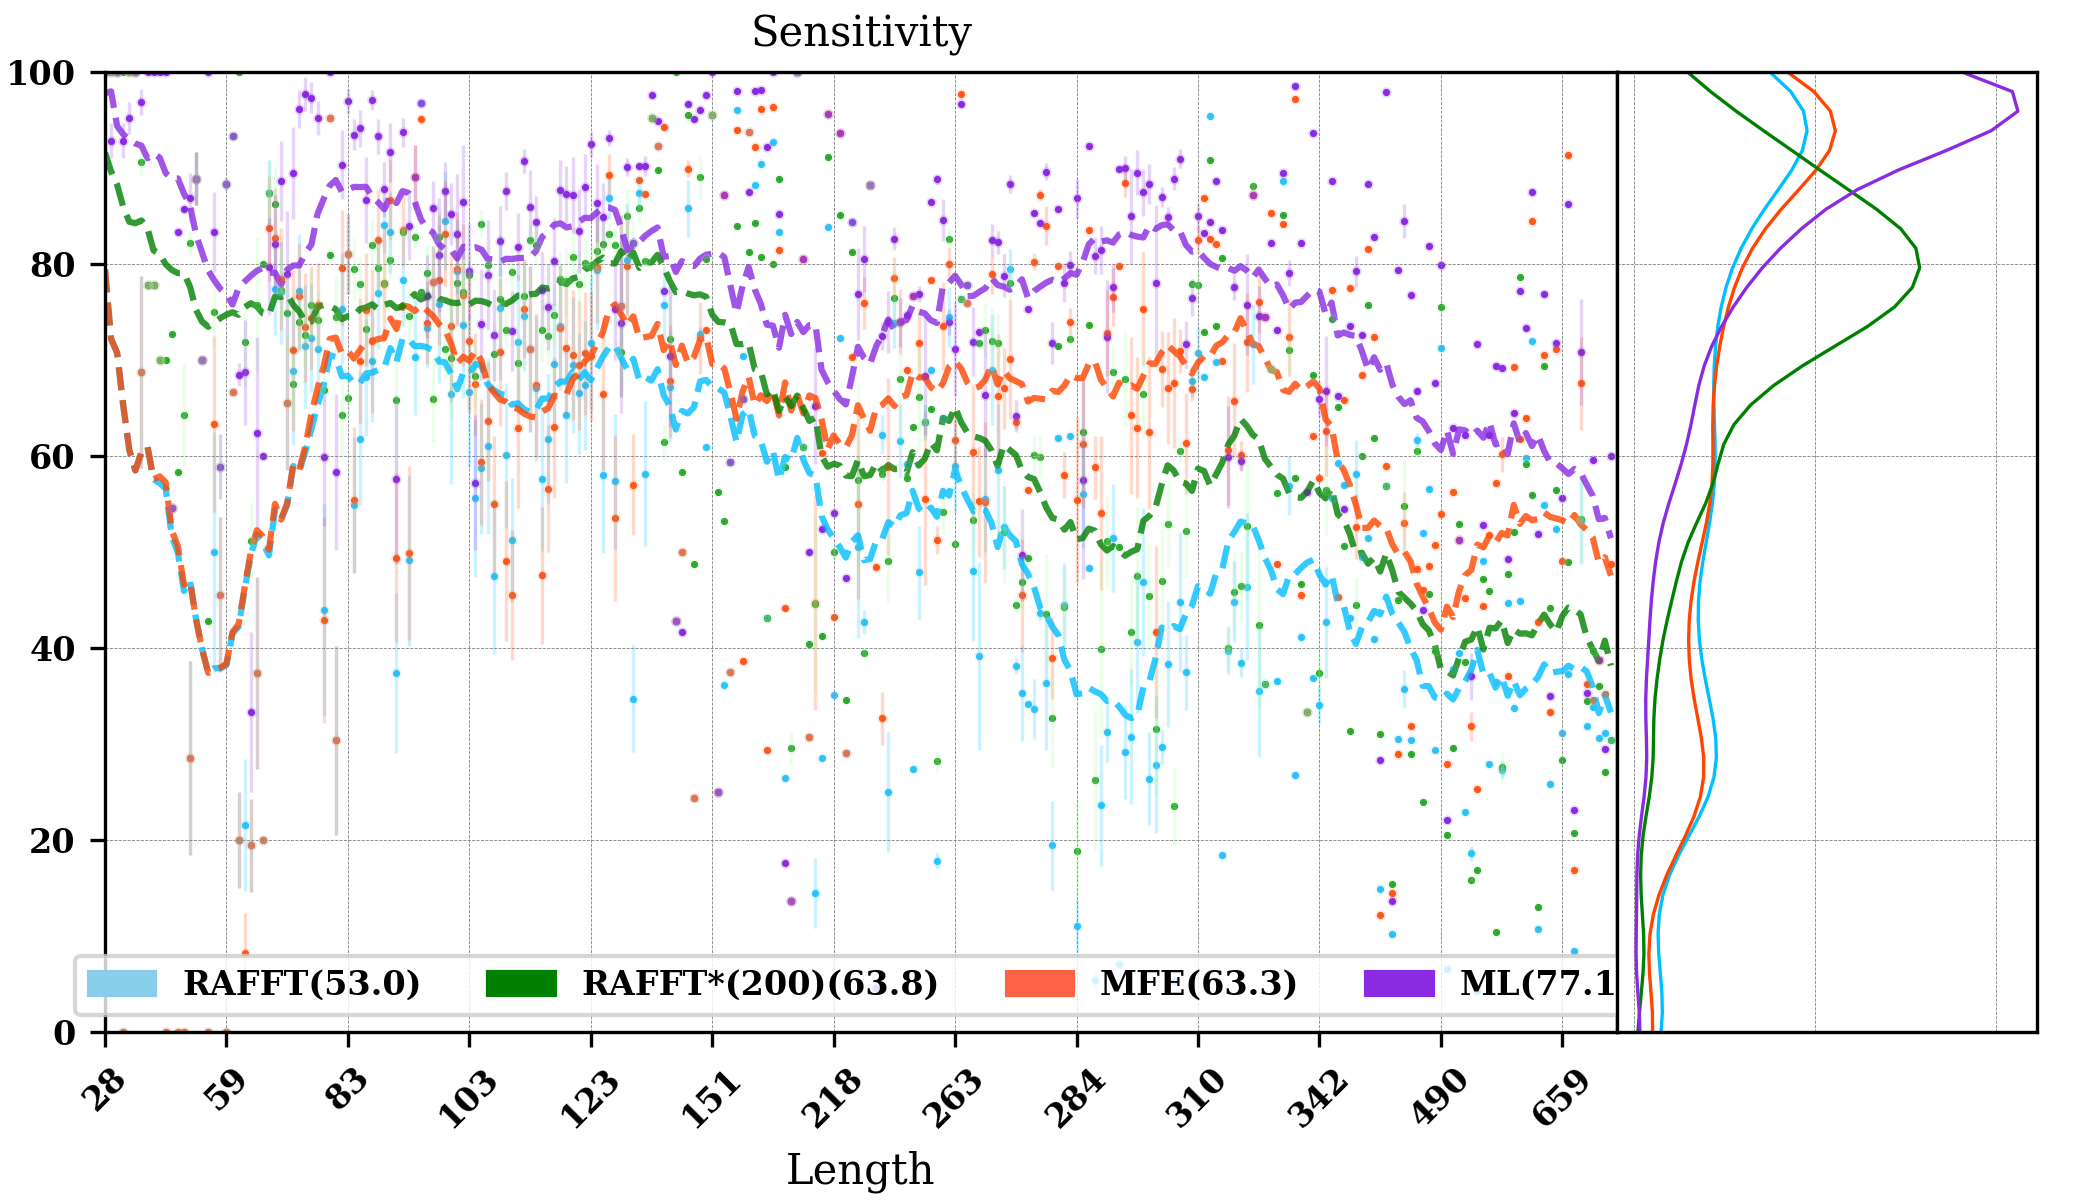
\includegraphics[scale=0.5]{img/fold_perf_sens_200.png}}
  \caption{\textbf{Predicted positive values and sensitivity results\label{perf_fig}.}
  RAFFT (blue) displayed the best energy found. RAFFT*(200) shows the best score found among 200 saved structures. Left pans show the density (sequence-wise) of the accuracy measures.}
\end{figure}

\begin{figure}[htbp]
\centering
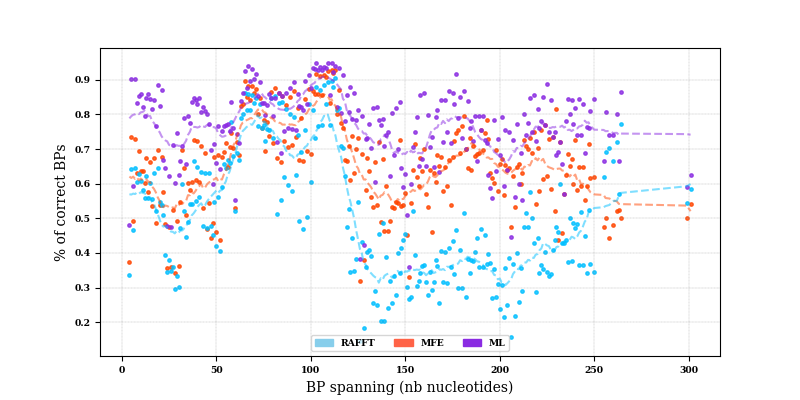
\includegraphics[width=.9\linewidth]{img/bp_spanning.png}
\caption{\textbf{Base pair spanning: It shows the percent of base pairs predicted found in the known structures per number of nucleotides between them.}}
\end{figure}

\begin{figure}[htbp]
\centering
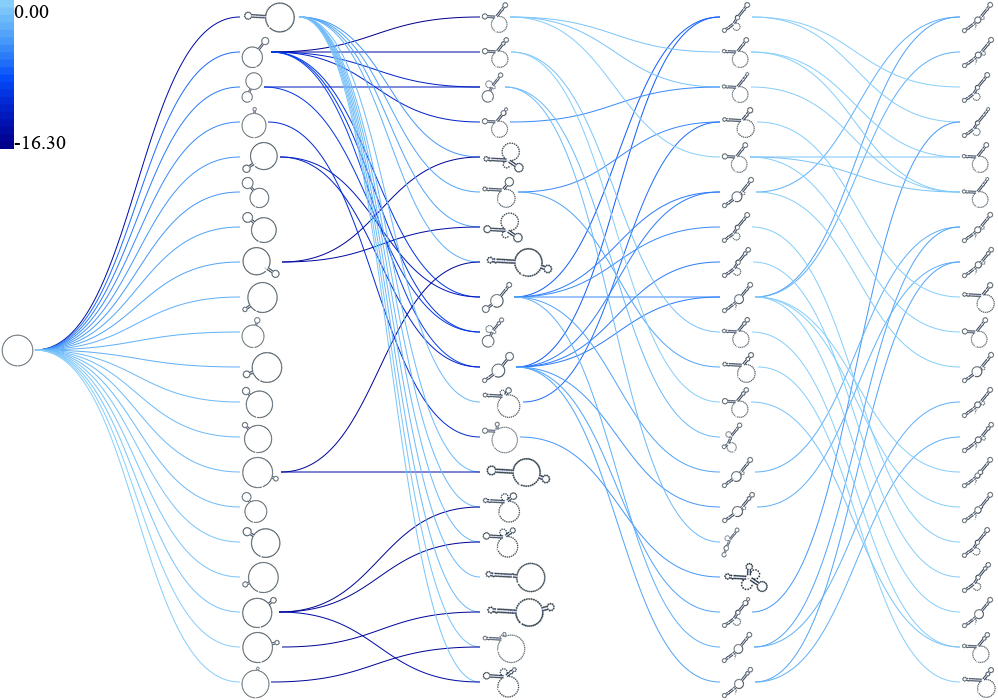
\includegraphics[width=.9\linewidth]{img/frame_shift/path_20.png}
\caption{\textbf{Fast-folding paths with 20 saved structures for the Coronavirus frameshifting stimulation element.}}
\end{figure}
\end{document}
